\documentclass[11pt, oneside]{article}   	% use "amsart" instead of "article" for AMSLaTeX format
%\usepackage{geometry}                		% See geometry.pdf to learn the layout options. There are lots.
%\geometry{letterpaper}                   		% ... or a4paper or a5paper or ... 
%\geometry{landscape}                		% Activate for rotated page geometry
%\usepackage[parfill]{parskip}    		% Activate to begin paragraphs with an empty line rather than an indent

\usepackage{geometry}
 \geometry{
 a4paper,
 total={170mm,257mm},
 left=20mm,
 top=15mm,
 }

\usepackage{graphicx}				% Use pdf, png, jpg, or eps§ with pdflatex; use eps in DVI mode
								% TeX will automatically convert eps --> pdf in pdflatex		
\usepackage{amssymb}
\usepackage{amsmath}
\usepackage{fancyhdr}
\usepackage[utf8]{inputenc}
\usepackage[english]{babel}
\usepackage{enumerate}
\usepackage{arcs}
\usepackage{cancel}
\usepackage{xfrac}
\usepackage{soul}
\usepackage{tikz}

%SetFonts

%SetFonts

\usepackage[inline]{asymptote}


\pagestyle{fancy}
\fancyhf{}
%\rhead{Teacher David @ 18601688612}
\lhead{\leftmark}


\title{Lecture Notes}
\author{Cindy Hu}
%\date{}							% Activate to display a given date or no date

\begin{document}
\maketitle




\section{Quadratic Equations}
\subsection{Solving Equations By Completing Square}
Given quadratic equation $ax^2+bx+c=0, a \ne 0, a, b, c \in \mathbb{R}$, we can solve it by the technique of \emph{Completing Square}: 
\begin{align*}
& ax^2+bx+c=0\\
\Rightarrow \quad & x^2+\frac{b}{a}x+\frac{c}{a}=0\\
\Rightarrow \quad & (x+\frac{b}{2a})^2-\frac{b^2}{4a^2}+\frac{c}{a}=0\\
%\Rightarrow \quad & (x+\frac{b}{2a})^2=\frac{b^2}{4a^2}-\frac{c}{a}\\
\Rightarrow \quad & (x+\frac{b}{2a})^2=\frac{b^2-4ac}{4a^2}\\
\Rightarrow \quad & x+\frac{b}{2a}=\pm \frac{\sqrt{b^2-4ac}}{2a}\\
\Rightarrow \quad & x=\frac{-b \pm \sqrt{b^2-4ac}}{2a}\\
\end{align*}

This is the formula commonly known for solving quadratic equations. Obviously, the equation has \hl{real solutions only if $b^2-4ac \ge 0$}. Specifically, \hl{when $b^2-4ac = 0$, the equation has two identical roots}. \\


\subsection{Factorisation}


If equation $ax^2+bx+c = 0$ has two roots $\alpha$ and $\beta$, then the equation can be \hl{factorised} as $a(x-\alpha)(\alpha-\beta)=0$. Therefore, if the equation can be easily factorised, we are able to solve it \hl{without using the formula introduced in the previous section}. 

For example, given equation $3x^2 - 8x +4=0$, if we want to factorise $3x^2 - 8x +4$, we firstly factorise the coefficient of the highest term $3x^2$, and factorise the constant term 4. For term $3x^2$, the coefficient is 3. It can be factorised as $1 \times 3$ or $-1\times -3$. For constant term 4, it can be factorised as $1 \times 4$, $-1\times -4$, $2\times 2$, or $-2\times -2$. 


\begin{figure}
\centering 
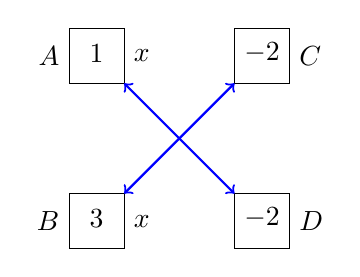
\begin{tikzpicture} [scale=0.7]

\draw (0,0) -- (0,1) -- (1,1) -- (1,0) -- cycle; 
\draw (3,0) -- (3,1) -- (4,1) -- (4,0) -- cycle; 
\draw (0,3) -- (0,4) -- (1,4) -- (1,3) -- cycle; 
\draw (3,3) -- (3,4) -- (4,4) -- (4,3) -- cycle; 

\draw [<->, blue, thick] (1,3)--(3,1);
\draw [<->, blue, thick] (1,1)--(3,3);

\coordinate [label=left:$A$](a) at(0, 3.5);
\coordinate [label=left:$B$](b) at(0, 0.5);
\coordinate [label=right:$C$](c) at(4, 3.5);
\coordinate [label=right:$D$](d) at(4, 0.5);

\coordinate [label=$1$](a1) at(0.5, 3.2);
\coordinate [label=$3$](b1) at(0.5, 0.2);
\coordinate [label=$-2$](c1) at(3.5, 3.2);
\coordinate [label=$-2$](d1) at(3.5, 0.2);

\coordinate [label=right:$x$](a2) at(1, 3.5);
\coordinate [label=right:$x$](b2) at(1, 0.5);

\end{tikzpicture}
\caption{Factorization of $3x^2 - 8x + 4$}
\label{fig:factorization}
\end{figure}


To make it illustrative, we usually use a \hl{square diagram} to fulfill the task.  As illustrated in Figure~\ref{fig:factorization}, we put the factors of 3 into squares $A$ and $B$, and put the factors of 4 into squares $C$ and $D$, we then cross-multiply $AD$ and $BC$ such that $AD + BC$ equals -8, the coefficient of the term $-8x$.  Figure~\ref{fig:factorization} illustrates the correct way to factorize $3x^2 -8x +4$. $AB$ implies that the term $3x^2$ is factorised as $x \times 3x$. $CD$ implies that 4 is factorised as $-2 \times -2$. $AC$ together means that we get $(x-2)$, $BD$ together means that we get $(3x-2)$. Eventually, $3x^2 - 8x +4 = (x-2)(3x-2)$. 

To solve $3x^2 - 8x +4=0$, we then have $x-2=0$ or $3x-2=0$. The two roots are $x=2$ and $x=\frac{2}{3}$. 

Unfortunately, not every quadratic equation can be factorised in such a clean way. But if we do meet an equation which we find can be factorised, solving it by factorisation would save quite a bit of effort. 




%\renewcommand{\labelenumii}{(\arabic{enumii})}


%\begin{enumerate}
%\renewcommand{\labelenumi}{1.\arabic{enumi}}

%\item \label{rule:add} \emph{Addition Principle}. If there are $a$ varieties of soup and $b$ varieties of salad, then there are $a+b$ possible ways to order a meal of soup \emph{or} salad (but not both soup and salad). 

%\end{enumerate}




\end{document} 